\documentclass[addpoints]{exam}
\usepackage{amsmath}
\usepackage{amsfonts}
\usepackage[most]{tcolorbox}
\usepackage{tikz}
\usepackage{pgfplots}
\usepackage{mdframed}
\usepackage{hyperref}
\usepackage{amsthm}

\marksnotpoints
\pointsinrightmargin
\bracketedpoints
\printanswers

\hypersetup{
  colorlinks=true,
  linkcolor=blue,
  filecolor=magenta,
  urlcolor=blue,
  pdfpagemode=FullScreen,
}

\urlstyle{same}

\pagestyle{headandfoot}
\firstpageheadrule
\runningheadrule
\firstpageheader{Pre Calc Prep}{Trig Functions and Identities}{Shah}
\runningheader{}{Trig}{}
\firstpagefooter{}{}{}
\runningfooter{ }{\thepage}{ }

\begin{document}
    \begin{tcolorbox}[breakable, title=TRIG FUNCTIONS REVIEW, colframe=black, sharp corners, colback=white, colbacktitle=white, coltitle=black]
        \Large \textbf{Review}
        \newline\normalsize Recall that the trigonometric functions are derived from the ratio of angles in a right triangle.  
        \vspace{0.1in}
        \newline
        \begin{minipage}{0.25\linewidth}
            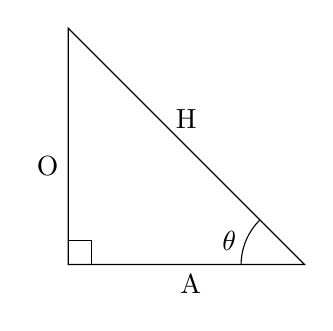
\begin{tikzpicture}
                \coordinate (A) at (0,0);
                \coordinate (B) at (0, 3);
                \coordinate (C) at (3, 0);

                \draw (A) -- (B) -- (C) -- cycle;

                \node[below left] at (0, 1.5) {O};
                \node[below right] at (1.3, 0) {A};
                \node [above] at (1.5, 1.6) {H};

                \draw (2.43,0.56) arc[start angle=135, end angle=180, radius=0.8cm] node[midway,left] {$\theta$};

                \draw (A) -- ++(0,0.3) -- ++(0.3,0) -- ++(0,-0.3);
            \end{tikzpicture}
        \end{minipage}
        \hfill
        \begin{minipage}{0.65\linewidth}
             Given the right triangle to the left, we can define the basic trigonometric functions as follows (fill in the blanks): \\
             \begin{minipage}{0.45\linewidth}
                 \begin{align*}
                     \sin\left(\theta\right) &= \frac{O}{H} \\
                     \cos\left(\theta\right) &= \frac{A}{H} \\ 
                     \tan\left(\theta\right) &= \frac{O}{A}
                 \end{align*}
             \end{minipage}
             \hfill
             \begin{minipage}{0.45\linewidth}
                \ifprintanswers
                    \begin{align*}
                        \csc\left(\theta\right) &= \frac{1}{\sin\left(\theta\right)} = \frac{H}{O} \\ 
                        \sec\left(\theta\right) &= \frac{1}{\cos\left(\theta\right)} = \frac{H}{A} \\ 
                        \cot\left(\theta\right) &= \frac{1}{\tan\left(\theta\right)} = \frac{A}{O}
                    \end{align*} 
                \else
                    \begin{align*}
                        \csc\left(\theta\right) &= \frac{1}{\sin\left(\theta\right)} = \frac{\phantom{H}}{\phantom{O}} \\ 
                        \sec\left(\theta\right) &= \frac{1}{\cos\left(\theta\right)} = \frac{\phantom{H}}{\phantom{A}} \\ 
                        \cot\left(\theta\right) &= \frac{1}{\tan\left(\theta\right)} = \frac{\phantom{A}}{\phantom{O}}
                    \end{align*} 
                \fi
             \end{minipage}
             \newline Note that $O$ stands for opposite, $A$ for adjacent, and $H$ for hypotenuse
        \end{minipage}
        \noindent\makebox[\linewidth]{\hrulefill}
        \vspace{0.1in}
        \newline \Large \textbf{Graphing}
        \newline\normalsize Complete the graphs below:
        \begin{questions}
            \question $f(x)=\sin(x)$ 
            \vspace{0.2in}
            \newline
            \begin{minipage}{0.45\linewidth}
                \ifprintanswers
                    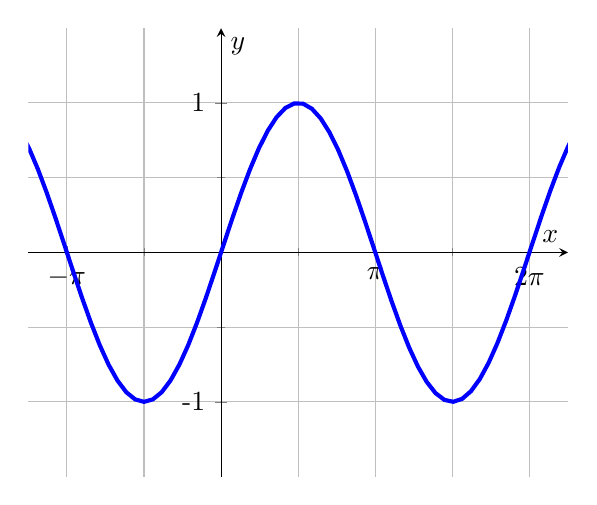
\begin{tikzpicture}
                        \begin{axis}[
                            grid=both,
                            axis lines = center,
                            xlabel={$x$},
                            ylabel={$y$},
                            minor tick num = 1,
                            xmin=-5*pi/4,
                            xmax=9*pi/4,
                            ymin=-1.5,
                            ymax=1.5,
                            xtick={-3.14159,0,3.14159,6.28318},
                            xticklabels={$-\pi$,0,$\pi$,$2\pi$},
                            ytick={-1,0,1},
                            yticklabels={-1, 0, 1},
                        ]

                        \addplot[samples=3000, line width=1.5pt, blue, domain=-180:360]{sin(deg(x))};
        
                        \end{axis}
                    \end{tikzpicture}
                \else
                    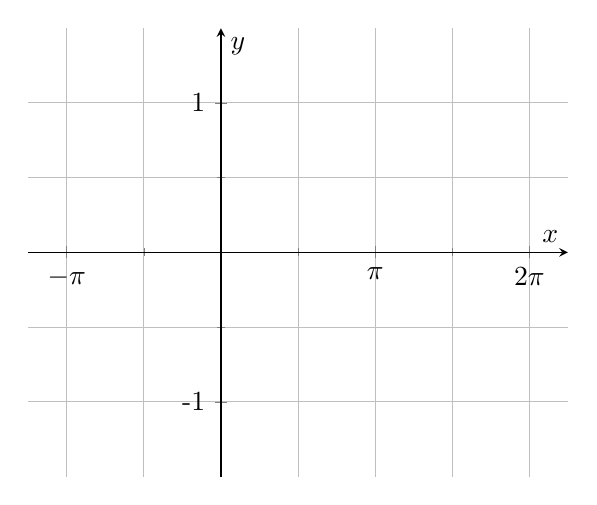
\begin{tikzpicture}
                        \begin{axis}[
                            grid=both,
                            axis lines = center,
                            xlabel={$x$},
                            ylabel={$y$},
                            minor tick num = 1,
                            xmin=-5*pi/4,
                            xmax=9*pi/4,
                            ymin=-1.5,
                            ymax=1.5,
                            xtick={-3.14159,0,3.14159,6.28318},
                            xticklabels={$-\pi$,0,$\pi$,$2\pi$},
                            ytick={-1,0,1},
                            yticklabels={-1, 0, 1},
                        ]
        
                        \end{axis}
                    \end{tikzpicture}
                \fi
            \end{minipage}
            \hfill 
            \begin{minipage}{0.45\linewidth}
                \begin{parts}
                    \part Period: 
                    \begin{solution}
                        $2\pi$
                    \end{solution}
                    \part Amplitude:
                    \begin{solution}
                        $1$
                    \end{solution}
                    \part Domain:
                    \begin{solution}
                        $(-\infty, \infty)$ OR $\mathbb{R}$
                    \end{solution}
                    \part Range:
                    \begin{solution}
                        $[-1, 1]$
                    \end{solution}
                \end{parts}
            \end{minipage}

            \newpage

            \question $f(x)=\cos(x)$
            \vspace{0.2in}
            \newline 
            \begin{minipage}{0.45\linewidth}
                \ifprintanswers
                    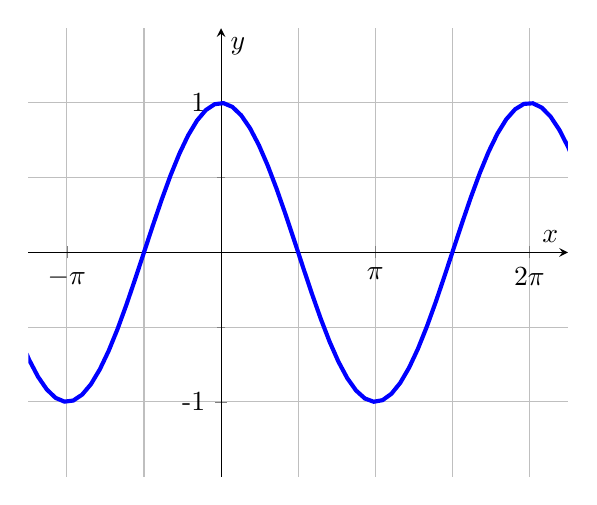
\begin{tikzpicture}
                        \begin{axis}[
                            grid=both,
                            axis lines = center,
                            xlabel={$x$},
                            ylabel={$y$},
                            minor tick num = 1,
                            xmin=-5*pi/4,
                            xmax=9*pi/4,
                            ymin=-1.5,
                            ymax=1.5,
                            xtick={-3.14159,0,3.14159,6.28318},
                            xticklabels={$-\pi$,0,$\pi$,$2\pi$},
                            ytick={-1,0,1},
                            yticklabels={-1, 0, 1},
                        ]

                        \addplot[samples=3000, line width=1.5pt, blue, domain=-180:360]{cos(deg(x))};
        
                        \end{axis}
                    \end{tikzpicture}
                \else
                    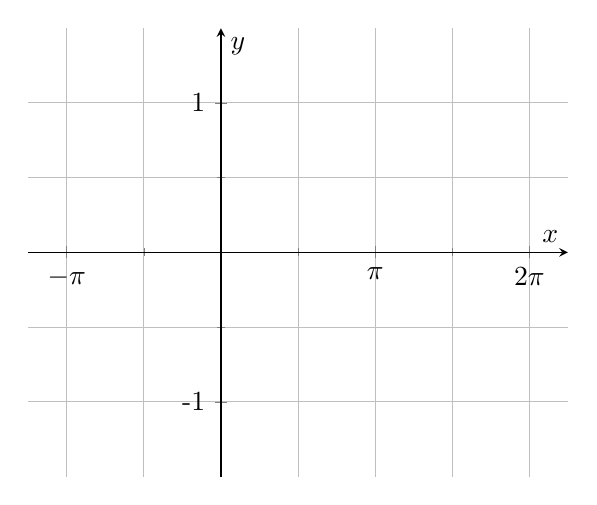
\begin{tikzpicture}
                        \begin{axis}[
                            grid=both,
                            axis lines = center,
                            xlabel={$x$},
                            ylabel={$y$},
                            minor tick num = 1,
                            xmin=-5*pi/4,
                            xmax=9*pi/4,
                            ymin=-1.5,
                            ymax=1.5,
                            xtick={-3.14159,0,3.14159,6.28318},
                            xticklabels={$-\pi$,0,$\pi$,$2\pi$},
                            ytick={-1,0,1},
                            yticklabels={-1, 0, 1},
                        ]
        
                        \end{axis}
                    \end{tikzpicture}
                \fi
            \end{minipage}
            \hfill 
            \begin{minipage}{0.45\linewidth}
                \begin{parts}
                    \part Period: 
                    \begin{solution}
                        $2\pi$
                    \end{solution}
                    \part Amplitude:
                    \begin{solution}
                        $1$
                    \end{solution}
                    \part Domain:
                    \begin{solution}
                        $(-\infty, \infty)$ OR $\mathbb{R}$
                    \end{solution}
                    \part Range:
                    \begin{solution}
                        $[-1, 1]$
                    \end{solution}
                \end{parts}
            \end{minipage}

            \question $f(x)=\tan(x)$ (Graph a single period)
            \vspace{0.2in}
            \newline
            \begin{minipage}{0.45\linewidth}
                \ifprintanswers
                    \begin{tikzpicture}
                        \begin{axis}[
                            grid=both,
                            axis lines = center,
                            xlabel={$x$},
                            ylabel={$y$},
                            minor tick num = 1,
                            xmin=-5*pi/4,
                            xmax=5*pi/4,
                            ymin=-1.5,
                            ymax=1.5,
                            xtick={-3.14159,0,3.14159},
                            xticklabels={$-\pi$,0,$\pi$},
                            ytick={-1,0,1},
                            yticklabels={-1, 0, 1},
                            unbounded coords = jump,
                            width=1.2\linewidth,
                            height=0.9\linewidth
                        ]

                        \addplot[samples=500, line width=1.5pt, blue, domain=-1*pi/2:1*pi/2]{tan(deg(x))};
        
                        \end{axis}
                    \end{tikzpicture}
                \else
                    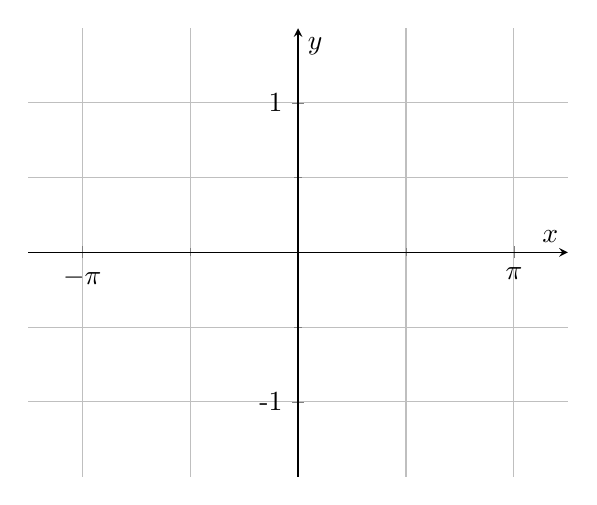
\begin{tikzpicture}
                        \begin{axis}[
                            grid=both,
                            axis lines = center,
                            xlabel={$x$},
                            ylabel={$y$},
                            minor tick num = 1,
                            xmin=-5*pi/4,
                            xmax=5*pi/4,
                            ymin=-1.5,
                            ymax=1.5,
                            xtick={-3.14159,0,3.14159},
                            xticklabels={$-\pi$,0,$\pi$},
                            ytick={-1,0,1},
                            yticklabels={-1, 0, 1},
                        ]
                        \end{axis}
                    \end{tikzpicture}
                \fi
            \end{minipage}
            \hfill 
            \begin{minipage}{0.45\linewidth}
                \begin{parts}
                    \part Period: 
                    \begin{solution}
                        $\pi$
                    \end{solution}
                    \part Domain:
                    \begin{solution}
                        \(\displaystyle\,(-\frac{n\pi}{2}, \frac{n\pi}{2})\, \forall n \in \mathbb{Z}\)
                    \end{solution}
                    \part Range:
                    \begin{solution}
                        $(-\infty, \infty)$ OR $\mathbb{R}$
                    \end{solution}
                    \part Vertical Asymptote:
                    \begin{solution}
                        $\displaystyle\,x=\frac{n\pi}{2}\,\forall n \in \mathbb{Z}$
                    \end{solution}
                \end{parts}
            \end{minipage}
            
            \ifprintanswers
                \textit{*Note that $\mathbb{Z}$ is the set of all integers}
            \fi
        \end{questions}
    \end{tcolorbox}

    \newpage 

    \begin{tcolorbox}[breakable, title=TRIG IDENTITIES, colframe=black, sharp corners, colback=white, colbacktitle=white, coltitle=black]
        \Large \textbf{Intro}
        \newline\normalsize A large part of what makes trig functions so important is their ability to be transformed from one function to another so easily. Knowing certain trig identities will make your mathematical life/career much easier in the near future. As well as having basic important identities memorized, being able to derive the truthfulness of an identity is also an important skill.
        \noindent\makebox[\linewidth]{\hrulefill}
        \vspace{0.1in}
        \newline\Large\textbf{Important Identities}
        \newline\normalsize These are the identities that you will see most often while solving problems, so it's important to recognize them and have them memorized: \\
        \begin{center}
            \textbf{Pythagorean Identities}
        \end{center}

        \begin{minipage}{0.3\linewidth}
            \[
            \sin^2\left(x\right) + \cos^2(x) = 1
            \]
        \end{minipage}
        \hfill
        \begin{minipage}{0.3\linewidth}
            \[
            1 + \cot^2(x) = \csc^2(x)
            \]
        \end{minipage}
        \hfill
        \begin{minipage}{0.3\linewidth}
           \[
            \tan^2(x) + 1 = \sec^2(x)
           \] 
        \end{minipage}
        \newline 
        \begin{center}
            \textbf{Double Angle Identities\small{*}}
        \end{center}
        \begin{minipage}{0.45\linewidth}
            \[
            \cos(2x)=\cos^2(x) - \sin^2(x)
            \]
        \end{minipage}
        \hfill
        \begin{minipage}{0.45\linewidth}
            \[
            \sin(2x)=2\sin(x)\cos(x)
            \]
        \end{minipage}
        \newline\textit{*Note that there are actually several different double angle identities for cosine, however, I recommend memorizing this form}
        \newline 
        \begin{center}
            \textbf{Half Angle Identities}
        \end{center}
        \begin{minipage}{0.45\linewidth}
            \[\displaystyle\,
            \sin^2(x)=\frac{1-\cos(2x)}{2}
            \]
        \end{minipage}
        \hfill
        \begin{minipage}{0.45\linewidth}
            \[\displaystyle\,
            \cos^2(x)=\frac{1+cos(2x)}{2} 
            \]
        \end{minipage}
        \noindent\makebox[\linewidth]{\hrulefill}
        \vspace{0.1in}
        \newline\Large\textbf{Proving Identities}
        \newline\normalsize When verifying trig identities its important to remember one key rule: \textbf{you cannot treat them as equations!!!} What this means is that you can't move terms from one side to another in order to reach a true statment, instead you must manipulate each side individually and independently until you can reach an equality by showing that both the left hand side and the right hand side of the equal sign are equivalent to the same quantity. 
        \newpage Now, for some practice use known trig identities and definitions to prove the following:
        \begin{questions}
            \question \(\displaystyle\, \frac{\sec x}{\cos x} - \frac{\tan x}{\cot x} = 1\)
            \begin{solution}[\stretch{1}]
                \begin{align*}
                    \frac{\sec x}{\cos x} - \frac{\frac{\sin x}{\cos x}}{\frac{\cos x}{\sin x}} &= 1 \\ 
                    \frac{1}{\cos^2} - \left(\frac{\sin x}{\cos x} \frac{\sin x}{\cos x}\right) &= 1 \\ 
                    \frac{1}{\cos^2 x} - \frac{\sin^2 x}{\cos^2 x} &= 1 \\ 
                    \frac{1 - \sin^2 x}{\cos^2 x} &= 1 \\ 
                    \frac{\cos^2 x}{\cos^2 x} &= 1 \\ 
                    1 &= 1
                \end{align*}
            \end{solution}
            \newpage
            \question \(\displaystyle\, \sec(x)-\tan(x)\sin(x) = \frac{1}{\sec(x)}\)
            \begin{solution}[\stretch{1}]
               \begin{align*}
                 \sec x - \tan x \sin x &= \frac{1}{\sec x} \\ 
                 \frac{1}{\cos x} - \frac{\sin x}{\cos x}\sin x &= \frac{1}{\sec x} \\ 
                 \frac{1}{\cos x} \left(1 - \sin^2 x\right) &= \frac{1}{\sec x} \\ 
                 \frac{1}{\cos x}\left(\cos^2 x\right) &= \frac{1}{\sec x} \\ 
                 \cos x &= \frac{1}{\sec x} \\ 
                 \frac{1}{\sec x} &= \frac{1}{\sec x}
               \end{align*}
            \end{solution}

            \question \(\displaystyle\, \frac{\sec x \sin x}{\tan x + \cot x} = \sin^2 x\)
            \begin{solution}[\stretch{1}]
              \begin{align*}
                \frac{\sec x \sin x}{\tan x + \cot x} &= \sin^2 x \\ 
                \frac{1}{\cos x}\frac{\sin x}{\tan x + \cot x} &= \sin^2 x \\ 
                \frac{\sin x}{\cos x\left(\tan x + \cot x\right)} &= \sin^2 x \\ 
                \frac{\sin x}{\cos x \left(\frac{\sin x}{\cos x} + \frac{\cos x}{\sin x}\right)}& = \sin^2 x \\ 
                \frac{\sin x}{\sin x + \frac{\cos^2 x}{\sin x}} &= \sin^2 x \\ 
                \frac{\sin x}{\frac{1}{\sin x}\left(\sin^2 x + \cos^2 x\right)} &= \sin^2 x \\ 
                \sin x\left(\frac{\sin x}{\sin^2 x + \cos^2 x}\right) &= \sin^2 x \\ 
                \sin x\left(\frac{\sin x}{1}\right) &= \sin^2 x \\ 
                \sin^2 x &= \sin^2 x
              \end{align*}
            \end{solution}
        \end{questions}
    \end{tcolorbox}
    \ifprintanswers
    \else 
    \newpage 
      \begin{center}
        \large\textbf{Use this page for your work}
      \end{center}
    \fi

    \newpage 
    \begin{align}
      a_c &= 2a_h \\ 
      m_{c}a_{c} &= F_t \\ 
      m_{h}a_{h} &= m_{h}g - 2F_t \\ 
      m_{h}\left(\frac{1}{2}a_c\right) &= m_{h}g-2m_{c}a_{c} \\ 
      \frac{1}{2}m_{h}a_{c} + 2m_{c}a_{c} &= m_{h}g \\ 
      a_c &= \boxed{\frac{m_{h}g}{\frac{1}{2}m_{h} + 2m_c}}
    \end{align}
\end{document}
